\documentclass{jps-cp}
\usepackage{txfonts} %Please comment out this line unless the txfonts package is availabe in your LaTeX system.
\usepackage{url}
\usepackage{multirow}
\usepackage{array, booktabs}
\usepackage{wrapfig}

\makeatletter
\newcommand{\figcaption}[1]{\def\@captype{figure}\caption{#1}}
\newcommand{\tblcaption}[1]{\def\@captype{table}\caption{#1}}

\title{New analysis method of TPC data using neural network}

\author{
  Takanobu \textsc{Doi}$^{1}$, Takahiro \textsc{Kawabata}$^{2}$, Tatsuya \textsc{Furuno}$^{3}$,
  Yuki \textsc{Fujikawa}$^{1}$, Kento \textsc{Inaba}$^{1}$, Motoki \textsc{Murata}$^{3}$,
  Shintaro \textsc{Okamoto}$^{1}$, and Akane \textsc{Sakaue}$^{1}$}

\inst{
  $^{1}$Department of Physics, Kyoto University, Kyoto, Kyoto 606-8502, Japan \\
  $^{2}$Department of Physics, Osaka University, Toyonaka, Osaka 540-0043, Japan \\
  $^{3}$Research Center for Nuclear Physics, Osaka University, Ibaraki, Osaka 567-0047, Japan }

\email{doi.takanobu.68x@st.kyoto-u.ac.jp}

\recdate{2019/8/31} % Write received date here

\abst{
  The MAIKo time projection chamber (TPC) enables us to project three-dimensional
  tracks of charged particles onto two planes perpendicular
  and parallel to the beam axis, and to acquire these projections as two images.
  It is, therefore, necessary to analyze these two-dimensional images to reconstruct the original three-dimensional tracks of the charged particles.
  Conventionally, we analyze them with the Hough transformation which is a method
  to find lines in images.
  This conventional method requires complex algorithms and a large computing power.
%  Recently neural networks have been widely employed for the image recognition.
  In the present work, we developed a new method to analyze track images obtained
  by the MAIKo TPC using neural networks which are widely employed for the image recognition.
  This new method successfully makes the analysis faster and more accurate than the conventional method.
%
%  TPC を用いた実験では荷電粒子の飛跡を測定することができる。
%  TPC では3次元的な荷電粒子の飛跡を2次元平面に射影した画像として得られるので、
%  データの解析には画像解析を行う必要がある。
%  従来はHough 変換を用いてデータの解析を行って来たが、
%  この方法を用いた解析には多くの労力を要する。
%  近年、画像データの認識にはニューラルネットワークが注目されている。
%  本研究では、新しくニューラルネットワークを用いた解析方法の開発を行った。
%  新しく開発した手法を用いることで、従来の方法と比較して高速に解析できるようになった。
} % Write abstract here

\kword{neural networks, time projection chamber (TPC), active target, MAIKo TPC} % Write keywords here

\begin{document}
\maketitle

\section{Introduction}
\begin{wrapfigure}{r}{15zw}
  \vspace{0zw}
  \centering
  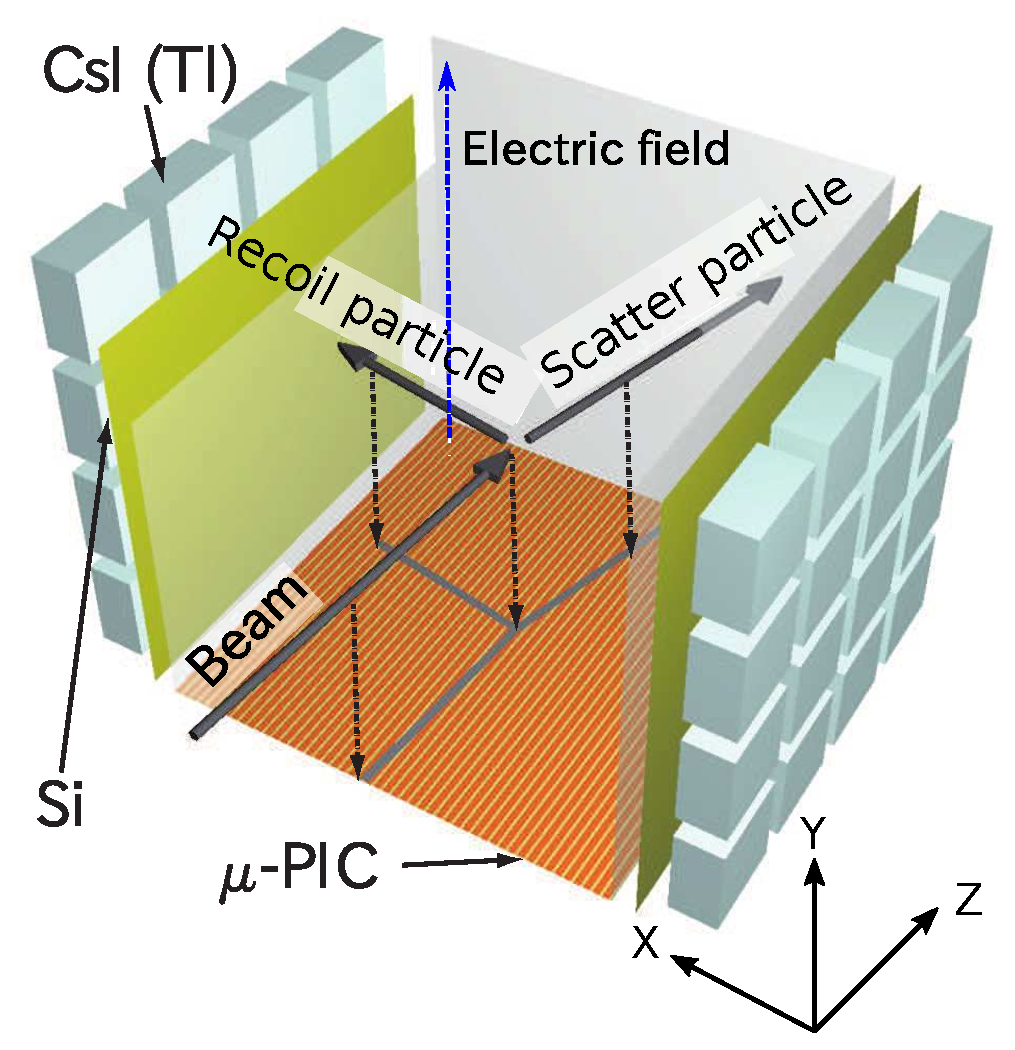
\includegraphics[clip, width=15zw]{eps/MAIKo.eps}
  \caption{Schematic view of the MAIKo TPC.}
  \label{fig:MAIKo}
  \vspace{-2zw}
\end{wrapfigure}
Time projection chambers (TPCs) are widely used to detect tracks of charged particles.
We developed a TPC using a micro pixel chamber ($\mu$-PIC)~\cite{mupic} named
MAIKo ($\mu$-PIC based active target for inverse kinematics.)~\cite{MAIKo}
for unstable nuclei experiments.
Figure \ref{fig:MAIKo} shows the schematic view of the MAIKo TPC.
When charged particles pass through the detection gas filled in the MAIKo TPC,
electrons are emitted along the particle tracks.
These electrons are drifted downward by an electric field and
gas-amplified on the surface of the $\mu$-PIC.
%
%近年、荷電粒子の飛跡を測定する検出器としてTime Projection Chamber (TPC) が
%広く用いられている。
%我々は不安定核実験のためにMicro Pixel Chamber ($\mu$-PIC)~\cite{mupic}を用いた
%Mu-Pic based Active target for Inverse Kinematics . (MAIKo) TPC~\cite{MAIKo}を開発した。
%MAIKo の概観図を Fig. \ref{fig:MAIKo} に示す。
%TPC は検出器にガスを充填しておき、荷電粒子がガス中を通過するときに発生する
%電子をドリフト電場 (上向き矢印) により読み出し面方向 (下向き) にドリフトさせる
%ことで飛跡を検出する。
The anode and cathode electrodes of the $\mu$-PIC are segmented into 256 strips 
which are arranged orthogonally.
These strips are aligned at 400-$\rm{\mu m}$ intervals.
Anode strips are parallel to $x$-axis and %は Fig. \ref{fig:MAIKo}のx軸の方向、
cathode strips are parallel to $z$-axis as shown in Fig.~\ref{fig:MAIKo}. %は z軸の方向と平行である。
Electrical signals induced by the amplified electrons and ions are read out through the anode and 
cathode strips to determine the $x$ and $z$ position of the particle tracks.
The vertical position of the tracks along the $y$-axis is determined 
from the drift time of the electrons.
Thus, the three-dimensional tracks are reconstructed from $x$-, $y$-, and $z$-coordinates.
%x, y, zの座標が決定できるので、飛跡を3次元的に再構成することが出来る。

%The MAIKo TPC is the active target whose detection gas is used as a target gas.
%Since incident particles are scattered by target particles in the sensitive volume of the TPC as shown in Fig.~\ref{fig:MAIKo}, 
%it is possible to detect low energy particles over a large solid angle.
Incident particles are scattered by target particles in the detection gas of the TPC as shown in Fig.~\ref{fig:MAIKo}, {\it i.e.} the detection gas plays a role of the target gas.
Scattered particles escape from the sensitive volume of the TPC and low-energy recoil particles stop inside.
Since reaction points are inside the sensitive volume of the TPC,
it is possible to detect low-energy particles over a large solid angle.
$\rm{H}_{2}$ or $\rm{He}$ gas is widely used as a target gas
but operation of TPC with pure $\rm{H}_{2}$ or $\rm{He}$ gas is unstable and prone to discharge.
Usually, quenching gas with a high tolerance for electric discharges
like $\rm{CO}_{2}$ or iso-butane is mixed with a target gas
for stable operation of the TPC although the quenching gas causes background events.
Recently, the elastic and inelastic alpha scattering on ${}^{10}\rm{C}$ were measured with the MAIKo TPC
at Research Center for Nuclear Physics (RCNP), Osaka University.
In this experiment, $\rm{He}$ (96\%) was used as the target gas, and $\rm{CO}_{2}$ (4\%) was used as the quenching gas.
%MAIKo TPC は検出ガスを散乱の標的として用いるアクティブ標的である。
%アクティブ標的では散乱が検出器内部で起こるため、大立体角で低エネルギー粒子の測定を行うことが可能となる。
%広く標的ガスとして用いられるのは $\rm{He}$ や $\rm{H}_{2}$であるが、
%これらのガスは放電耐性が低いので、
%通常は放電耐性の高い $\rm{CO}_{2}$ やイソブタンをクエンチングガスとして
%混合させてTPC を運用する。
%このとき、クエンチングガスからの散乱は背景事象となる。
%近年、大阪大学核物理研究センター (RCNP) において、
%MAIKo TPC を用いた${}^{10}\rm{C}$と${}^{4}\rm{He}$の非弾性散乱の測定が初めて行われた。
%この実験では標的ガスである$\rm{He}$ (96\%)に、$\rm{CO}_{2}$ (4\%)をクエンチングガスとして
%混合して測定を行った。

The tracks of charged particles in each event were projected onto the two planes that are perpendicular to the anode and cathode strips, and were recorded as the anode and cathode images.
%The MAIKo TPC outputs two images in each event.
Figures \ref{fig:true} and \ref{fig:false} are examples of the acquired images.
These black-and-white images with $1024\times 256$ pixels present the hit pattern of the 256 strips on the anode and cathode recorded
at every $10~\rm{ns}$ for the duration of $10~\rm{ns}\times 1024 = 10.24~\rm{\mu s}$.
Figure \ref{fig:true} shows a ${}^{10}\rm{C}+\alpha$ event
in which the incident ${}^{10}\rm{C}$ beam was scattered at the small angle from the beam axis and the $\alpha$ particle was
recoiled at the large angle.
On the other hand, Fig.~\ref{fig:false} shows a background event due to the quenching gas
in which the incident ${}^{10}\rm{C}$ beam was scattered at the large angle off a heavy nucleus.

%MAIKo TPC において荷電粒子の飛跡は、
%anode strip に垂直な面に射影された画像 (anode image) と
%cathode strip に垂直な面に射影された画像 (cathode image) の2つの画像として取得される。
%$\mu$-PIC の anode and cathode strips は256 本あり、
%信号波高の時間変化は100 MHz で1,024 samples 測定されるので、
%取得される画像の解像度は256 $\times$ 1,024 pixels となる。
%Figures \ref{fig:true} and \ref{fig:false} はRCNPで行われた実験で取得された
%データの一例である。
%Figure \ref{fig:true} は$\rm{He}$ガスと散乱した事象、
%Fig. \ref{fig:false} はクエンチングガスと散乱した事象である。
For the ${}^{10}\rm{C}+\alpha$ events, the energy and emission angle of the recoil $\alpha$ particle must
be determined to obtain the spectroscopic information such as the excitation energy of ${}^{10}\rm{C}$
and the scattering angle in the center-of-mass system.
The energy of the recoil $\alpha$ particle is determined from the length of the track in the detection gas consisting of the target gas and the detection gas,
while the emission angle is determined from the opening angle between the incident particle and the recoil $\alpha$ particle.
To analyze the anode and cathode images, there are two steps.
\begin{itemize}
\item
  Select ${}^{10}\rm{C}+\alpha$ events form background events.
\item
  Determine the length and the emission angle of the recoil $\alpha$ particle from anode and cathode images.
\end{itemize}
%散乱実験では、散乱粒子のエネルギーと放出角度を決定する必要がある。
%散乱粒子のエネルギーは散乱粒子がガス中で停止するまでの飛跡の長さから、
%放出角度は散乱前後の粒子の飛跡から決定することが出来る。
%飛跡情報の抽出を行うためには
%\begin{itemize}
%\item 標的との散乱事象と背景事象との選別
%\item 飛跡の長さや方向などの物理的情報の抽出
%\end{itemize}
%の大きくわけて2つの解析が必要になる。
However, the conventional analysis method requires a lot of efforts to select events and determine tracks from the anode and cathode images.
Therefore, we needed to develop a new analysis method using neural networks which are widely employed for the image recognition in recent years.
%Figures \ref{fig:true} and \ref{fig:false} のような画像データに対して、
%事象の選別や飛跡情報の抽出には多くの労力が必要となる。
%そこで、我々は近年画像認識において多くの成果を出している
%ニューラルネットワークを用いることで、
%より高速な解析を行うことが出来る解析方法の開発を行った。

\begin{figure}
  \centering
  \begin{minipage}{0.45\columnwidth}
    \centering
    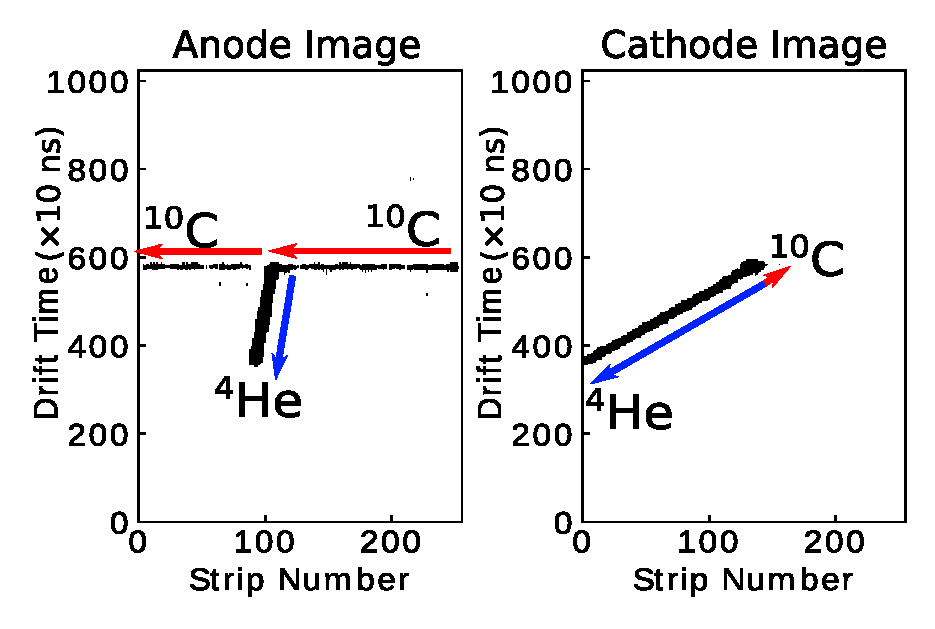
\includegraphics[clip, width=0.9\columnwidth]{eps/true.eps}
    \caption{Typical anode and cathode images recorded in a ${}^{10}\rm{C}+\alpha$ event}
    \label{fig:true}
  \end{minipage}
  \hfill
  \begin{minipage}{0.45\columnwidth}
    \centering
    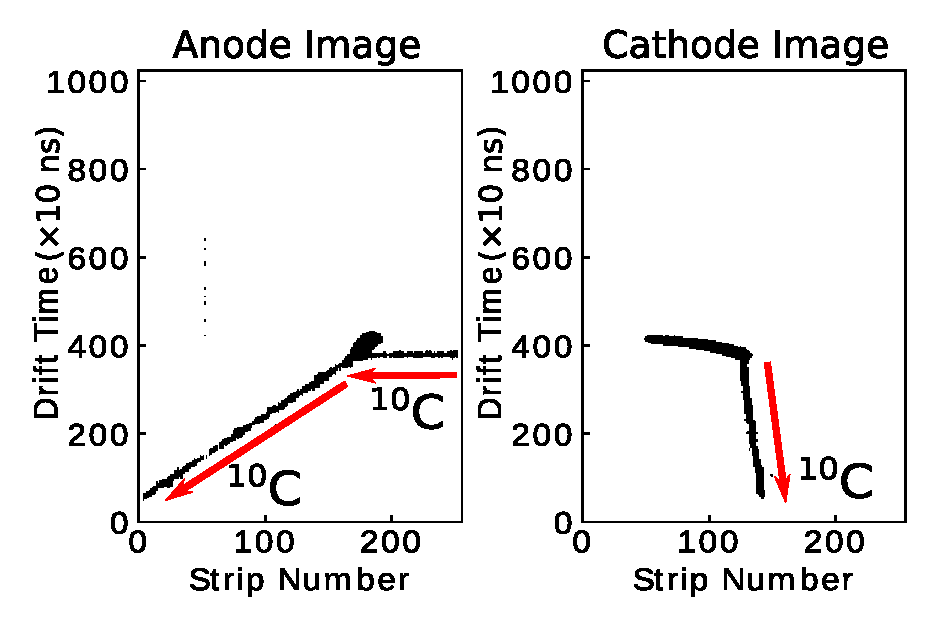
\includegraphics[clip, width=0.9\columnwidth]{eps/false.eps}
    \caption{Same with Fig.~\ref{fig:true} but recorded in a background event.}
    \label{fig:false}
  \end{minipage}
\end{figure}

\section{Conventional method}
The conventional method employs the Hough transformation in order to
select the ${}^{10}\rm{C}+\alpha$ events and to determine tracks.
The Hough transformation is one of methods to find lines from an image.
%従来は、得られたデータから背景事象の除去を行うために、
%画像中の直線を抽出する手法の1つである
%Hough 変換を用いたアルゴリズムによって行ってきた。
In the Hough transformation, a hit pixel at $(x_{i}, y_{i})$ in the image
is transformed into
a curved line in the $(\theta, r)$ parameter space (Hough space)
according to Eq. (\ref{eq:real2hough}).
\begin{equation}
  \label{eq:real2hough}
  r = x_{i}\cos\theta+y_{i}\sin\theta. 
\end{equation}
A point at $(\theta_{j}, r_{j})$ in the Hough space corresponds to a straight line
in the original image as given by Eq. (\ref{eq:hough2real}).
\begin{equation}
  \label{eq:hough2real}
  y = -\frac{x}{\tan\theta_{j}}+\frac{r_{j}}{\sin\theta_{j}}. 
\end{equation}
When the pixels in the anode or cathode image lie on a straight line,
their transformed curves intersect at one point at $(\theta_{j}, r_{j})$ in the Hough space.
Thus, the intersection point in the Hough space gives the particle track according to Eq. (\ref{eq:hough2real}).

It is possible to select the ${}^{10}\rm{C}+\alpha$ events by
utilizing information about the straight lines extracted from the anode and cathode images such as
the number, position, angle and length.
Once the ${}^{10}\rm{C}+\alpha$ events are selected, the energy and angle of the recoil $\alpha$ particle
are determined from the images to calculate the excitation energy and the scattering angle in the center-of-mass system.
However, the conventional method with the Hough transformation requires a complicated algorithm with many adjustable parameters,
and the optimization of these parameters needs a large computing power.
%抽出した直線の長さや角度、本数、配置に対して多くの条件を課すことによって、
%$\rm{He}$との散乱事象を選別することが出来る。
%さらに、選別された事象における$\rm{He}$の飛跡の長さや角度から、
%散乱角とエネルギーを決定することが出来る。
%しかし、事象選別に必要な条件には複雑な分岐を必要とし、
%多くのパラメータを導入しなければならない。
%そのため、パラメータの最適化や画像識別に多くの時間を必要とする。
It takes about 24 hours to optimize the parameters using 100 CPUs
in the computing system at RCNP, 
and about one second to process the anode and cathode images from one event using one CPU after the parameter optimization.
The accuracy of the event selection was rated 89\% using 3,000 events,
which were tagged with human eyes.
%パラメータの最適化には100 CPU を使用して約1日かかり、
%その後の画像識別には1 eventあたり1秒かかった。
%この手法による識別能力の評価には、画像データを人間が目で見て
%散乱事象もしくは背景事象と判断した3,000イベントを評価用データとして用いて行った。
%全事象のうち、散乱事象または背景事象の区別を正しく判断することが
%出来た事象数の割合を正解率としたとき、この従来型の解析手法では89\%の正解率であった。

\section{New method}
The conventional method has problems of requiring the complex algorithm and a large computing power.
We developed a new method using neural networks.
Using neural networks, it might be possible to recognize images
considering many features of tracks without any complicated algorithms.
Once a neural network trained, the neural network is expected to recognize images faster and more accurate than the conventional method.

%従来手法では識別に複雑な分岐条件や多くの計算機パワー
%が必要になるという問題点があった。
%そこで、我々は近年注目されているニューラルネットワークを用いることで、
%これらの問題点を克服する新しい解析方法の開発を試みた。
%ニューラルネットワークを用いることで、複雑な条件分岐を導入することなく、
%直線の位置、角度などの従来の解析手法ではまとめて扱うことの難しい
%多くの特徴量を同時に考慮した画像識別が可能になるかもしれない。
%また、ニューラルネットワークは一度構築するとその後は短時間で画像識別を行うことができる。
%このようなニューラルネットワークの特徴を活かすことで、
%従来のアルゴリズムでは実現が難しかった高い精度と短い識別時間を実現することが期待される。

\vspace{0zw}
\begin{figure}
  \centering
  \begin{minipage}{0.4\columnwidth}
    \centering
    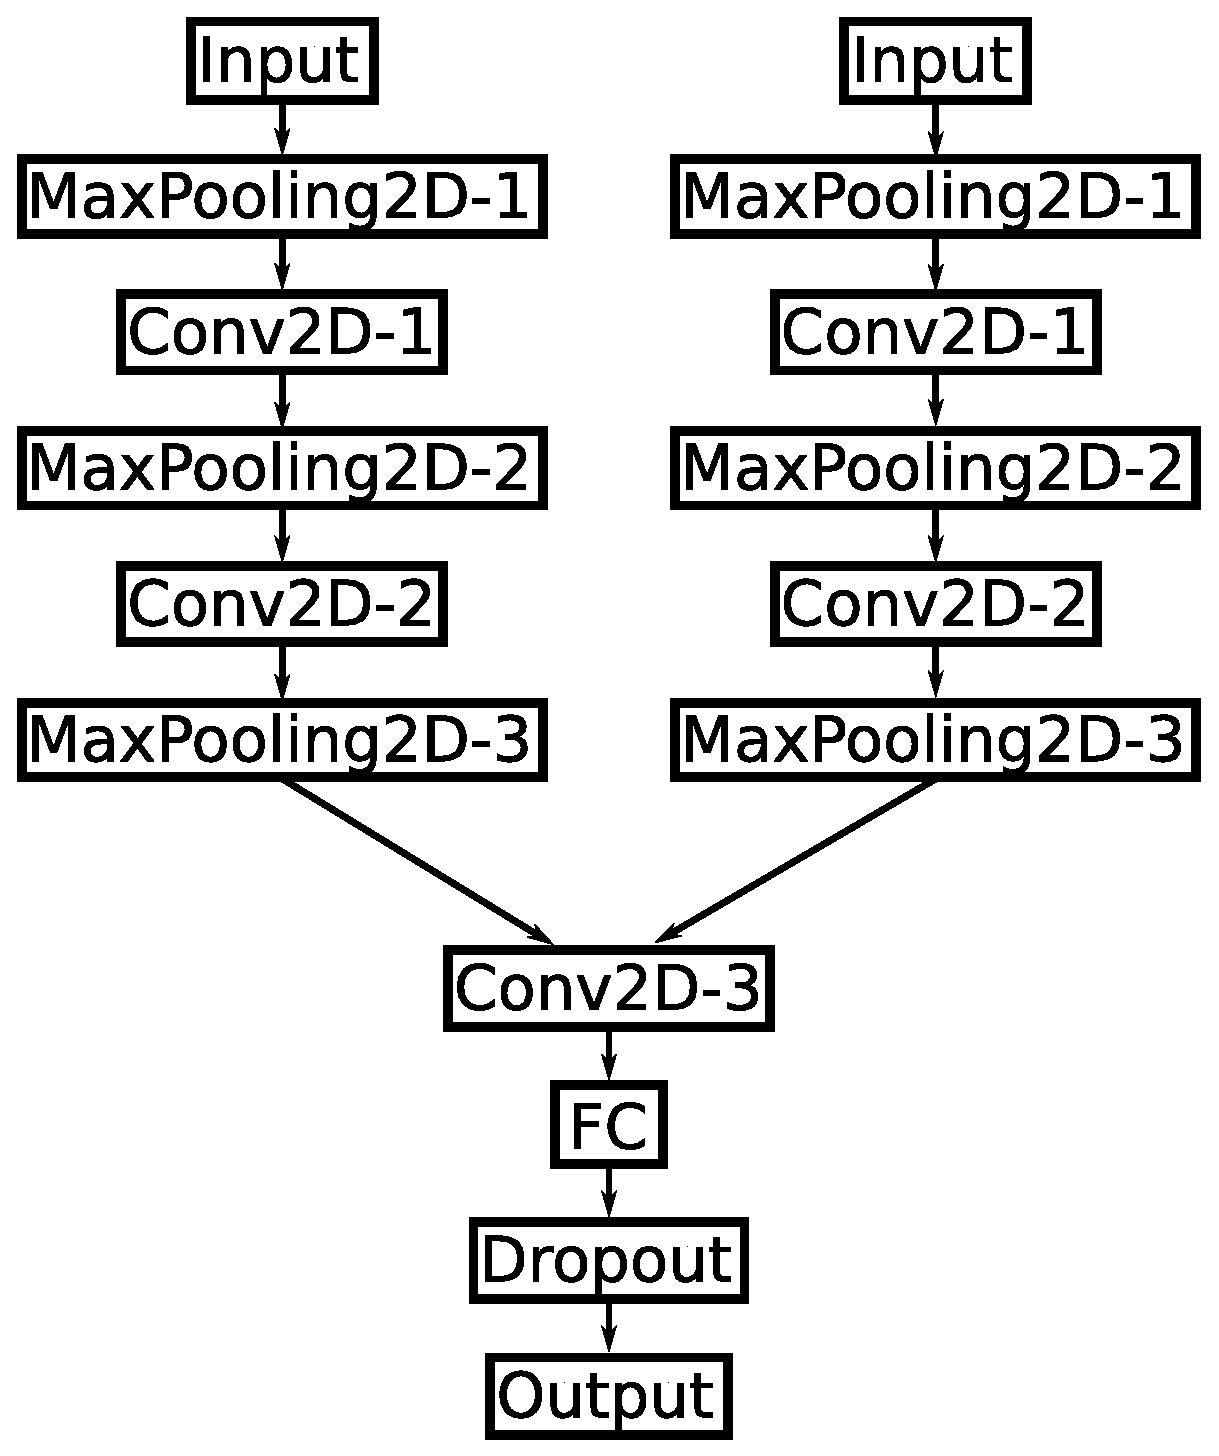
\includegraphics[clip, width=0.9\columnwidth]{eps/event_selection.eps}
%    \caption{データの選別を行うためのニューラルネットワーク}
    \caption{Schematic structure of the neural network for the event selection.}
    \label{fig:selection}
  \end{minipage}
  \hfill
  \begin{minipage}{0.4\columnwidth}
    \centering
    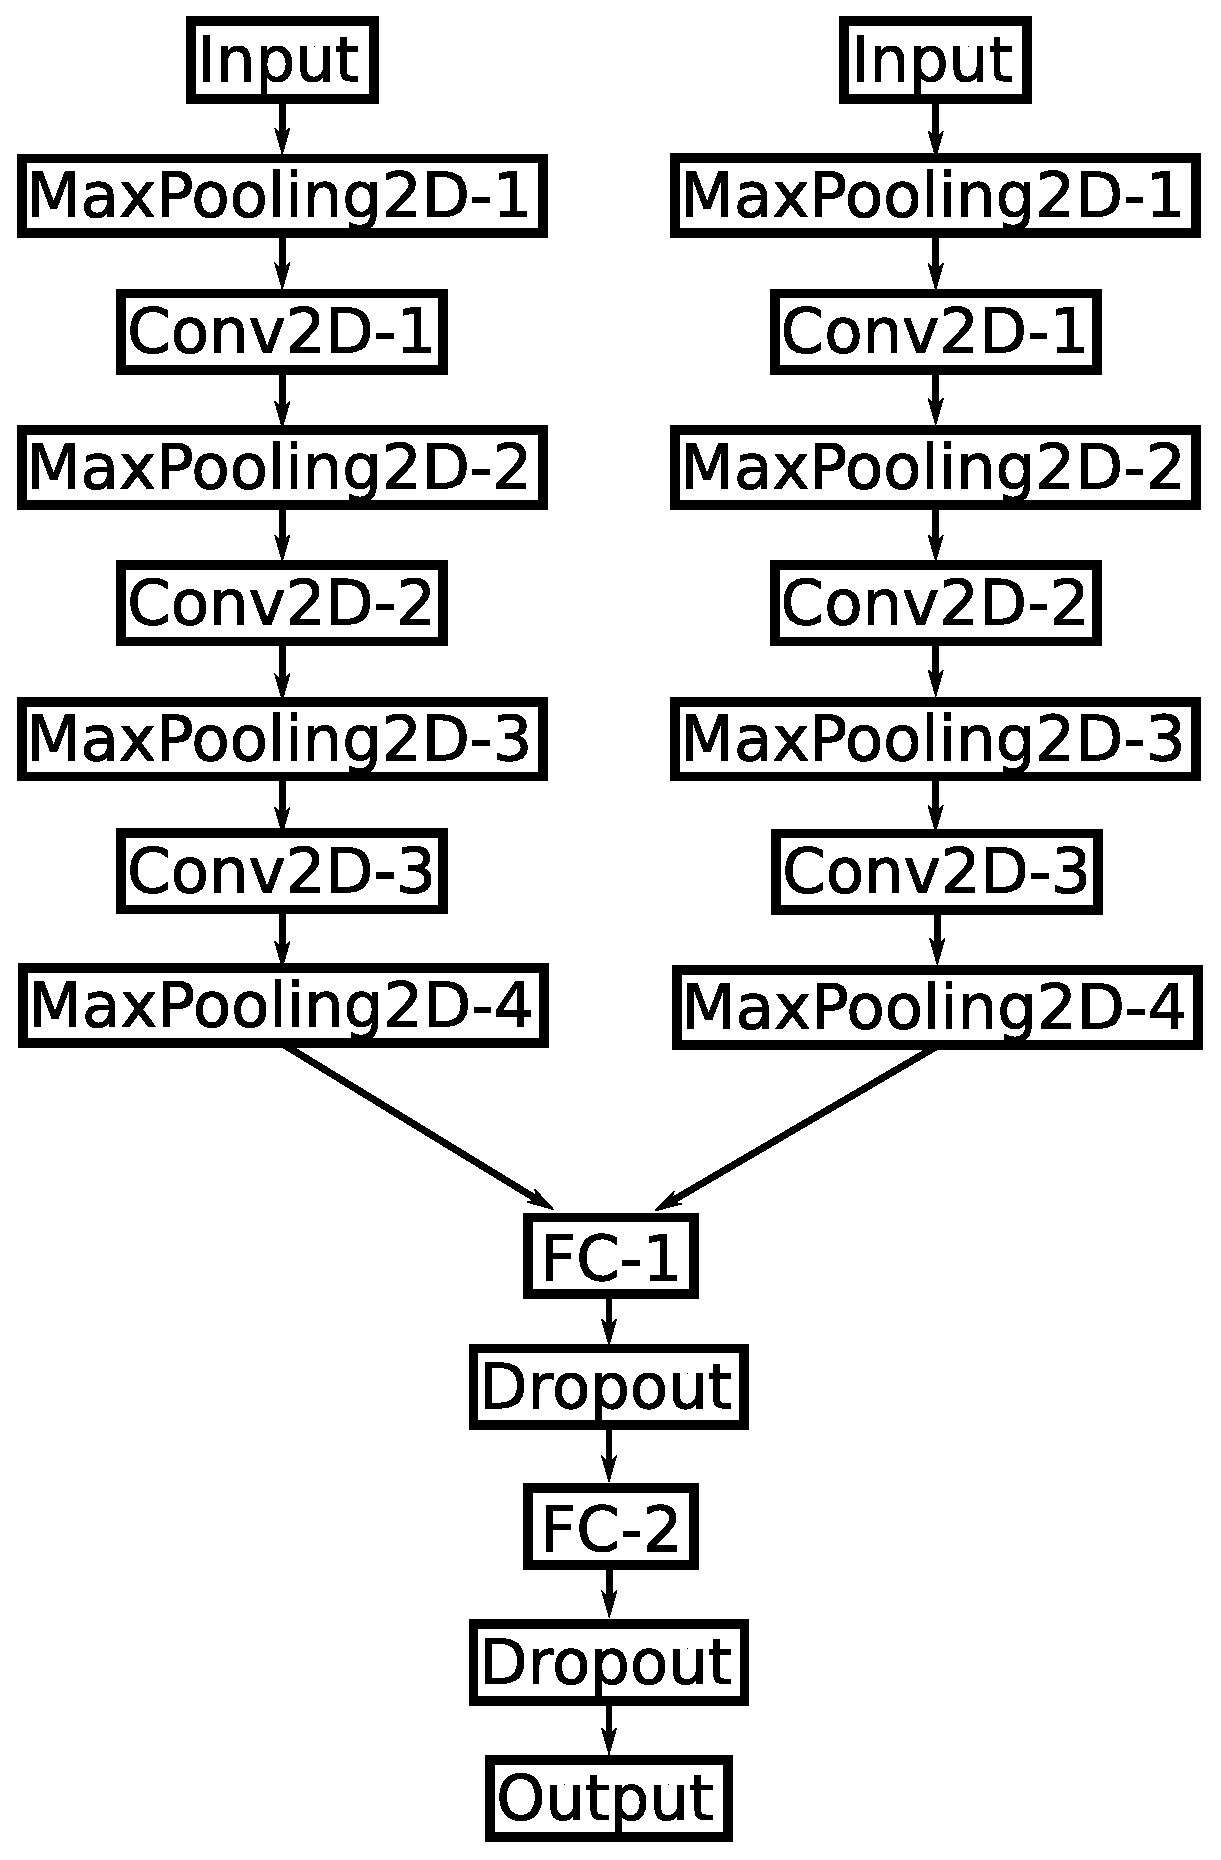
\includegraphics[clip, width=0.9\columnwidth]{eps/point_detection.eps}
%    \caption{画像から情報を抽出するためのニューラルネットワーク}
    \caption{Schematic structure of the neural network for the track determination.}
    \label{fig:extraction}
  \end{minipage}
\end{figure}

We used convolutional neural networks (CNNs) that are useful for image recognition~\cite{lenet,alexnet},
because the data from the MAIKo TPC are images.
%CNN is the network that has convolutional layers.%<-- この行は何も追加情報がないと言われた
Since the analysis consists of the event selection and the track determination,
we used two networks to analyze.
Figures \ref{fig:selection} and \ref{fig:extraction} show
the networks for the event selection and the track determination, respectively.
Because the anode and cathode images have different features,
the networks have two branches.
We inputted a pair of images from the MAIKo TPC to the neural networks.
The network for the event selection has 16 layers and the network for the track determination has 21 layers.
``Input'', ``MaxPooling2D'', ``Conv2D'', ``FC'', and ``Output'' in Figs. \ref{fig:selection} and \ref{fig:extraction} mean
the input layer, maxpooling layer, convolutional layer, full connection layer, and output layer respectively.
%MAIKo TPC から得られるデータが画像であるため、画像認識に有用とされる
%Convolutional Neural Network (CNN)~\cite{lenet,alexnet} を用いた。
%CNN とはネットワーク内に畳み込み層を有するネットワーク構造である。
%解析には事象の選別と飛跡情報の抽出の2つの段階があるため、
%2種類のニューラルネットワークを用いて解析を行った。
%事象の選別を行うニューラルネットワークと
%画像から飛跡情報を抽出するニューラルネットワークの構造を
%それぞれFigs. \ref{fig:selection} and \ref{fig:extraction}に示す。

In the event selection, we obtained a probability that the pair of images were taken
in the ${}^{10}\rm{C}+\alpha$ event.
If the probability was larger than 50\%, the event was regarded as the ${}^{10}\rm{C}+\alpha$ scattering.
This network was trained and evaluated with the images tagged by eye scan,
which were used in the conventional analysis.
The 2,700 events were used for the training, and the other 300 events were for the evaluation.
%事象選別のためのニュラルネットワークは、MAIKo TPC から得られる2つの画像を入力し、
%その事象が標的と散乱した事象である確率を出力する。
%出力された確率が50\%以上である場合にその事象を標的と散乱した事象であるとした。
%anode image と cathode image では飛跡が異なる特徴を持つため、
%2つの入力が別れた構造を持つネットワークを構築した。
%人間が判断したデータを用いて、学習および評価を行った。
%学習には2,700 events、評価には300 events を使用した。
In the track determination, the network outputted the coordinates of two endpoints of
a track of a recoil $\alpha$ particle in a ${}^{10}\rm{C}+\alpha$ event in which the recoil $\alpha$ particle stopped
in the sensitive volume of the MAIKo TPC.
This network was trained and evaluated with the images processed by the conventional method.
The 3,012 events were used for the training, and the other 1,554 events were for the evaluation.
%飛跡情報を抽出するためのネットワークには、
%事象選別のときと同様に MAIKo TPC から得られる2つの飛跡画像を入力し、
%散乱が起こった座標と反跳した${}^{4}\rm{He}$が停止した座標を出力させる。
%%%%学習を効率的に行うために、出力される座標は各軸が0--1の範囲になるように規格化した座標系で得られる。
%%%%このネットワークは21層からなり、2入力1出力の形をしている。
%教師データには従来手法で決定した座標を用いた。
%学習には3,012 events、評価には1,554 events を使用した。

We used Intel Core i7, Nvidia GeForce GTX 1080Ti, Ubuntu 18.04 LTS, and
TensorFlow~\cite{tensorflow} + Keras~\cite{keras} in the present analysis.
%学習環境はIntel Core i7、Nvidia GeForce GTX 1080Ti、Ubuntu 18.04 LTS、
%TensorFlow~\cite{tensorflow}+Keras~\cite{keras} を用いた。

\section{Result}
\begin{wrapfigure}{r}{25zw}
  \vspace{-6zw}
  \centering
  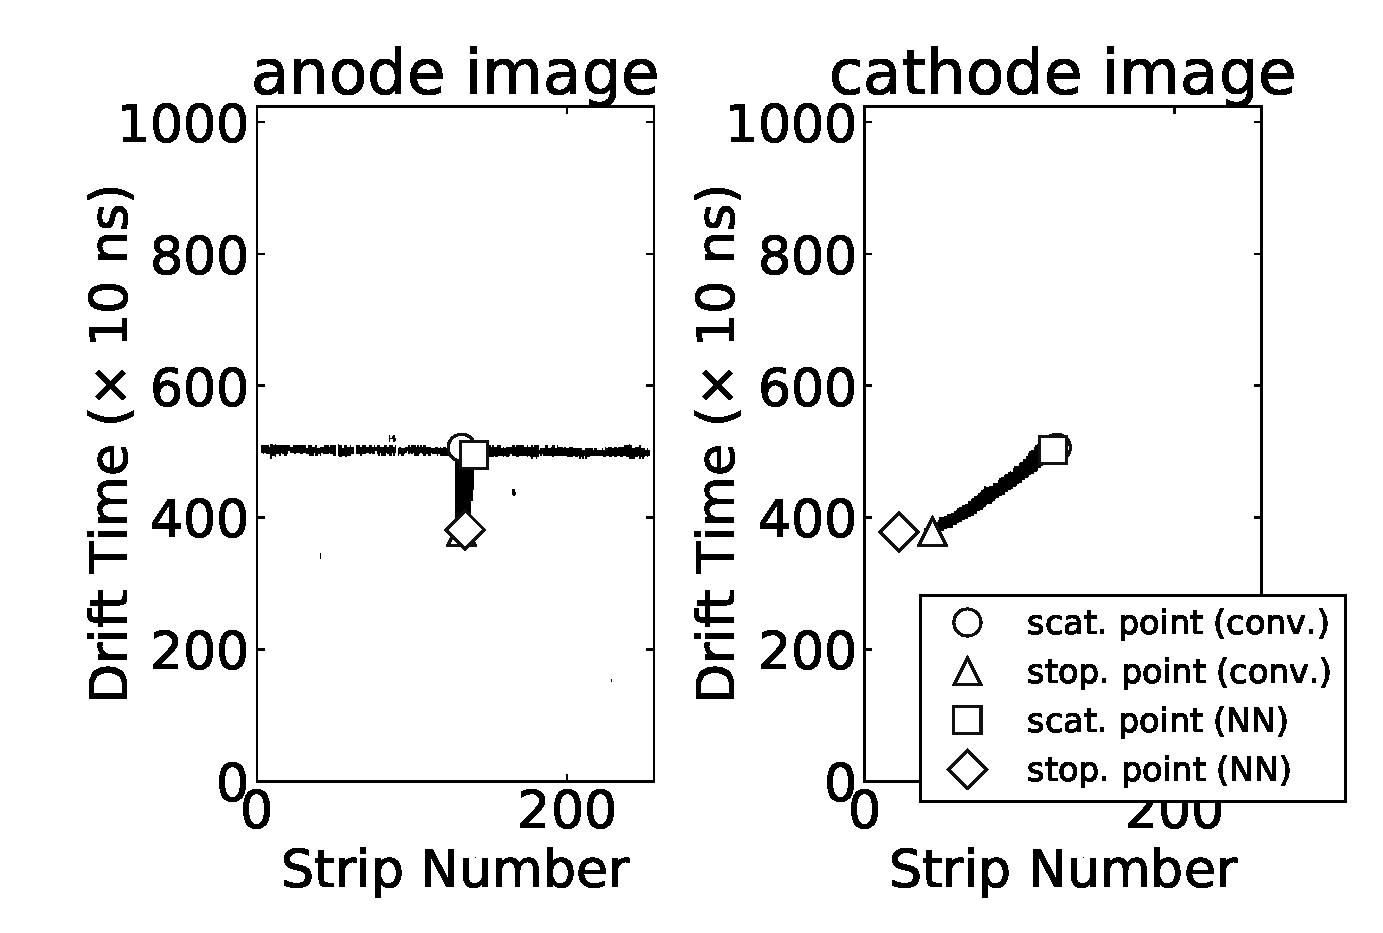
\includegraphics[clip, width=25zw]{eps/compare_mono_v2.eps}
%  \caption{ニューラルネットワークによって決定した座標とHough変換によって決定した座標との比較}
  \caption{Comparison of the track endpoints determined by the conventional method and the neural network.}
  \label{fig:result_detection}
  \vspace{-2zw}
\end{wrapfigure}

The neural network for the event selection was trained 200 times for the 2,700 events.
It took about 26 minutes for the training and about one second to process for the 300 events.
The accuracy of the event selection by the neural network was 96\%,
while the accuracy by the conventional method was 89\%.
The neural network is able to select events faster and more accurate than the conventional method.

%事象選別のためのニューラルネットワークは、2,700 events に対して200 回学習を行った。
%学習にはおよそ26分、その後の推測には300 events に対しておよそ1秒かかった。
%従来手法の評価に用いたのと同じ実験データのうち、300 eventsを用いて評価を行った結果、
%正解率は96\%であった。
%従来の手法と比較して高精度に事象選別を行うことが可能となった。
%また、パラメータチューニングおよび選別に要する時間も大きく短縮することができた。

The neural network for the track determination was trained 500 times for the 3,012 events.
It took about 270 minutes for the training and about two seconds to process the 1,554 events.
The track endpoints in a typical event determined by the neural network are compared with those
by the conventional method in Fig.~\ref{fig:result_detection}.
The circles and triangles show the scattering and the stopping points determined by the conventional method,
while the squares and rhombuses show those determined by the neural network.
The differences in the coordinates of the track endpoints determined by the conventional method
and the neural network are about four mm in the standard deviation for the 1,554 events.
The processing time for the neural network to find the track endpoints was much shorter than the conventional method.
%座標の決定のためのニューラルネットワークは、3,012 events に対して500 回学習を行った。
%学習にはおよそ270分、その後の推測には1,554 events に対しておよそ2秒かかった。
%典型的なイベントにおいて、
%学習後にニューラルネットワークが予測した座標と従来手法によって決定した座標の比較をFig. \ref{fig:result_detection} に示す。
%学習データの散乱が起こった点を円、反跳粒子が停止した点を三角で示す。
%学習後に推論によって決定した散乱が起こった点を四角、反跳粒子が停止した点をひし形で示す。
%従来手法とニューラルネットワークを用いた手法のそれぞれで決定した座標は、
%ほぼ一致している。
%1,554 events に対して学習に用いた点とニューラルネットワークを用いて決定した点のズレは、
%平均二乗誤差で約4 mm となった。
%従来の手法と比較してパラメータチューニングおよび情報の抽出にかかる時間を短縮することができた。


\section{Conclusion}
We developed a new method with neural networks to analyze the track images acquired by the MAIKo TPC.
It was found that this new method made the event selection and the track determination faster and more accurate
than the conventional method with the Hough transformation.
%従来のHough 変換を用いた画像識別アルゴリズムに替わる、
%ニューラルネットワークを用いた新手法の開発を行った。
%新手法は従来のものよりも高速かつ高精度に事象の選別を行うことが可能となった。
%また、飛跡情報の抽出については従来の精度を保ちつつ、高速に行うことが可能となった。
%ニューラルネットワークを用いた解析手法はTPC の解析に有用であることがわかった。

\begin{thebibliography}{9}
\bibitem{mupic}
  A.~Ochi, T.~Nagayoshi, T.~Tanimori, T.~Nagae, and M.~Nakamura,
  Nucl. Instrum. Methods Phys. Res. A \textbf{471}, 264 (2001).
\bibitem{MAIKo}
  T.~Furuno, T.~Kawabata, H.~Ong, S.~Adachi, Y.~Ayyad, T.~Baba, Y.~Fujikawa, T.~Hashimoto, K.~Inaba, Y.~Ishii,
  S.~Kabuki, H.~Kubo, Y.~Matsuda, Y.~Matsuoka, T.~Mizumoto, T.~Morimoto, M.~Murata, T.~Sawano, T.~Suzuki, A.~Takada,
  J.~Tanaka, I.~Tanihata, T.~Tanimori, D.~Tran, M-, Tsumura, and H.~Watanabe,
  Nucl. Instrum. Methods Phys. Res. A \textbf{908}, 215 (2018).
\bibitem{lenet}
  Y.~LeCun, L.~Bottou, Y.~Bengio, and P.~Haffner,
  Proceedings of the IEEE \textbf{86}, 11, 2278 (1998).
\bibitem{alexnet}
  Alex~Krizhevsky, Ilya~Sutskever, and Geoffrey~E.~Hinton,
  Proceedings of the 25th International Conference on Neural Information Processing Systems - Volume \textbf{1}, 1097 (2012).
%\bibitem{tensorflow}
%  A.~Davis, J.~Dean, M.~Devin, S.~Ghemawat, I.~Goodfellow, A.~Harp, G.~Irving,
%  M.~Isard, Y.~Jia, R.~Jozefowicz, L.~Kaiser, M.~Kudlur, J.~Levenberg,
%  D.~Man\'{e}, R.~Monga, S.~Moore, D.~Murray, C.~Olah, M.~Schuster, J.~Shlens,
%  B.~Steiner, I.~Sutskever, K.~Talwar, P.~Tucker, V.~Vanhoucke, V.~Vasudevan,
%  F.~Vi\'{e}gas, O.~Vinyals, P.~Warden, M.~Wattenberg, M.~Wicke, Y.~Yu, and
%  X.~Zheng, (2015).
%  \url{https://tensorflow.org}
\bibitem{tensorflow}
  Mart\'{\i}n~Abadi,
  Ashish~Agarwal,
  Paul~Barham,
  Eugene~Brevdo,
  Zhifeng~Chen,
  Craig~Citro,
  Greg~S.~Corrado,
  Andy~Davis,
  Jeffrey~Dean,
  Matthieu~Devin,
  Sanjay~Ghemawat,
  Ian~Goodfellow,
  Andrew~Harp,
  Geoffrey~Irving,
  Michael~Isard,
  Yangqing Jia,
  Rafal~Jozefowicz,
  Lukasz~Kaiser,
  Manjunath~Kudlur,
  Josh~Levenberg,
  Dan~Man\'{e},
  Rajat~Monga,
  Sherry~Moore,
  Derek~Murray,
  Chris~Olah,
  Mike~Schuster,
  Jonathon~Shlens,
  Benoit~Steiner,
  Ilya~Sutskever,
  Kunal~Talwar,
  Paul~Tucker,
  Vincent~Vanhoucke,
  Vijay~Vasudevan,
  Fernanda~Vi\'{e}gas,
  Oriol~Vinyals,
  Pete~Warden,
  Martin~Wattenberg,
  Martin~Wicke,
  Yuan~Yu, and
  Xiaoqiang~Zheng.
  {{TensorFlow}: Large-Scale Machine Learning on Heterogeneous Systems},
  2015.
  Software available from \url{tensorflow.org/}.
\bibitem{keras}
  F.~Chollet et al., (2015). \url{https://keras.io}
%\bibitem{vgg}
%  K.~Simonyan, and A.~Zisserman
%  arXiv:1409.1556 [cs] (2014).
%
  
%\bibitem{cp} The abbreviation for JPS Conference Proceedings should be ``JPS Conf. Proc." in the reference list.
%\bibitem{jpsj} The abbreviation for the Journal of the Physical Society of Japan should be ``J. Phys. Soc. Jpn." in the reference list.
%\bibitem{ptep} The abbreviation for the Progress of Theoretical and Experimental Physics should be ``Prog. Theor. Exp. Phys." in the reference list.
%\bibitem{instructions} More abbreviations of journal titles are listed in ``Instructions for Preparation of Manuscript", which is available at our Web site (http://jpsj.jps.or.jp).
%\bibitem{format} F. Author, S. Author, and T. Author, Abbreviated journal title \textbf{volume in bold face}, initial page or article number (year of publication).
\end{thebibliography}

\end{document}

